% Created by tikzDevice version 0.6.2-92-0ad2792 on 2013-03-31 12:43:04
% !TEX encoding = UTF-8 Unicode
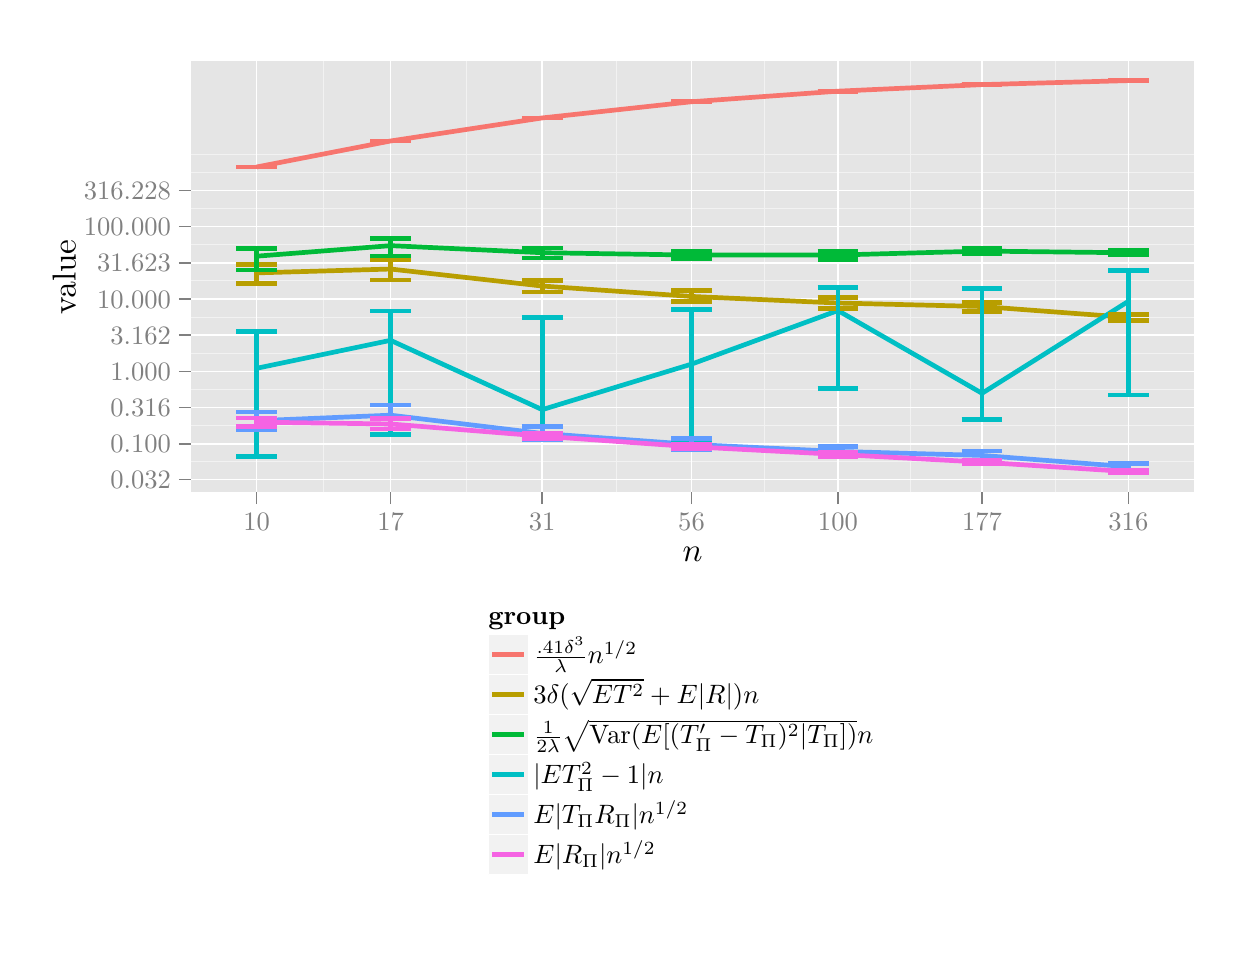
\begin{tikzpicture}[x=1pt,y=1pt]
\definecolor[named]{fillColor}{rgb}{1.00,1.00,1.00}
\path[use as bounding box,fill=fillColor,fill opacity=0.00] (0,0) rectangle (433.62,325.21);
\begin{scope}
\path[clip] (  0.00,  0.00) rectangle (433.62,325.21);
\definecolor[named]{drawColor}{rgb}{1.00,1.00,1.00}
\definecolor[named]{fillColor}{rgb}{1.00,1.00,1.00}

\path[draw=drawColor,line width= 0.6pt,line join=round,line cap=round,fill=fillColor] (  0.00,  0.00) rectangle (433.62,325.21);
\end{scope}
\begin{scope}
\path[clip] ( 58.88,157.27) rectangle (421.57,313.17);
\definecolor[named]{fillColor}{rgb}{0.90,0.90,0.90}

\path[fill=fillColor] ( 58.88,157.27) rectangle (421.57,313.17);
\definecolor[named]{drawColor}{rgb}{0.95,0.95,0.95}

\path[draw=drawColor,line width= 0.3pt,line join=round] ( 58.88,168.36) --
	(421.57,168.36);

\path[draw=drawColor,line width= 0.3pt,line join=round] ( 58.88,181.37) --
	(421.57,181.37);

\path[draw=drawColor,line width= 0.3pt,line join=round] ( 58.88,194.45) --
	(421.57,194.45);

\path[draw=drawColor,line width= 0.3pt,line join=round] ( 58.88,207.54) --
	(421.57,207.54);

\path[draw=drawColor,line width= 0.3pt,line join=round] ( 58.88,220.62) --
	(421.57,220.62);

\path[draw=drawColor,line width= 0.3pt,line join=round] ( 58.88,233.71) --
	(421.57,233.71);

\path[draw=drawColor,line width= 0.3pt,line join=round] ( 58.88,246.79) --
	(421.57,246.79);

\path[draw=drawColor,line width= 0.3pt,line join=round] ( 58.88,259.87) --
	(421.57,259.87);

\path[draw=drawColor,line width= 0.3pt,line join=round] ( 58.88,272.89) --
	(421.57,272.89);

\path[draw=drawColor,line width= 0.3pt,line join=round] ( 58.88,279.37) --
	(421.57,279.37);

\path[draw=drawColor,line width= 0.3pt,line join=round] (106.92,157.27) --
	(106.92,313.17);

\path[draw=drawColor,line width= 0.3pt,line join=round] (158.53,157.27) --
	(158.53,313.17);

\path[draw=drawColor,line width= 0.3pt,line join=round] (212.91,157.27) --
	(212.91,313.17);

\path[draw=drawColor,line width= 0.3pt,line join=round] (266.33,157.27) --
	(266.33,313.17);

\path[draw=drawColor,line width= 0.3pt,line join=round] (318.82,157.27) --
	(318.82,313.17);

\path[draw=drawColor,line width= 0.3pt,line join=round] (371.30,157.27) --
	(371.30,313.17);
\definecolor[named]{drawColor}{rgb}{1.00,1.00,1.00}

\path[draw=drawColor,line width= 0.6pt,line join=round] ( 58.88,161.88) --
	(421.57,161.88);

\path[draw=drawColor,line width= 0.6pt,line join=round] ( 58.88,174.83) --
	(421.57,174.83);

\path[draw=drawColor,line width= 0.6pt,line join=round] ( 58.88,187.91) --
	(421.57,187.91);

\path[draw=drawColor,line width= 0.6pt,line join=round] ( 58.88,201.00) --
	(421.57,201.00);

\path[draw=drawColor,line width= 0.6pt,line join=round] ( 58.88,214.08) --
	(421.57,214.08);

\path[draw=drawColor,line width= 0.6pt,line join=round] ( 58.88,227.17) --
	(421.57,227.17);

\path[draw=drawColor,line width= 0.6pt,line join=round] ( 58.88,240.25) --
	(421.57,240.25);

\path[draw=drawColor,line width= 0.6pt,line join=round] ( 58.88,253.33) --
	(421.57,253.33);

\path[draw=drawColor,line width= 0.6pt,line join=round] ( 58.88,266.42) --
	(421.57,266.42);

\path[draw=drawColor,line width= 0.6pt,line join=round] ( 82.72,157.27) --
	( 82.72,313.17);

\path[draw=drawColor,line width= 0.6pt,line join=round] (131.13,157.27) --
	(131.13,313.17);

\path[draw=drawColor,line width= 0.6pt,line join=round] (185.93,157.27) --
	(185.93,313.17);

\path[draw=drawColor,line width= 0.6pt,line join=round] (239.88,157.27) --
	(239.88,313.17);

\path[draw=drawColor,line width= 0.6pt,line join=round] (292.78,157.27) --
	(292.78,313.17);

\path[draw=drawColor,line width= 0.6pt,line join=round] (344.86,157.27) --
	(344.86,313.17);

\path[draw=drawColor,line width= 0.6pt,line join=round] (397.74,157.27) --
	(397.74,313.17);
\definecolor[named]{drawColor}{rgb}{0.97,0.46,0.43}

\path[draw=drawColor,line width= 1.7pt,line join=round] ( 82.72,274.86) --
	(131.13,284.26) --
	(185.93,292.59) --
	(239.88,298.44) --
	(292.78,302.26) --
	(344.86,304.63) --
	(397.74,306.08);
\definecolor[named]{drawColor}{rgb}{0.72,0.62,0.00}

\path[draw=drawColor,line width= 1.7pt,line join=round] ( 82.72,236.60) --
	(131.13,237.99) --
	(185.93,231.85) --
	(239.88,228.09) --
	(292.78,225.71) --
	(344.86,224.45) --
	(397.74,220.50);
\definecolor[named]{drawColor}{rgb}{0.00,0.73,0.22}

\path[draw=drawColor,line width= 1.7pt,line join=round] ( 82.72,242.63) --
	(131.13,246.44) --
	(185.93,243.89) --
	(239.88,243.04) --
	(292.78,243.06) --
	(344.86,244.48) --
	(397.74,243.87);
\definecolor[named]{drawColor}{rgb}{0.00,0.75,0.77}

\path[draw=drawColor,line width= 1.7pt,line join=round] ( 82.72,202.12) --
	(131.13,212.23) --
	(185.93,187.18) --
	(239.88,203.63) --
	(292.78,222.99) --
	(344.86,193.09) --
	(397.74,226.33);
\definecolor[named]{drawColor}{rgb}{0.38,0.61,1.00}

\path[draw=drawColor,line width= 1.7pt,line join=round] ( 82.72,183.17) --
	(131.13,185.18) --
	(185.93,178.58) --
	(239.88,174.62) --
	(292.78,172.09) --
	(344.86,170.64) --
	(397.74,166.54);
\definecolor[named]{drawColor}{rgb}{0.96,0.39,0.89}

\path[draw=drawColor,line width= 1.7pt,line join=round] ( 82.72,182.66) --
	(131.13,182.00) --
	(185.93,177.60) --
	(239.88,173.78) --
	(292.78,171.00) --
	(344.86,168.21) --
	(397.74,164.78);
\definecolor[named]{drawColor}{rgb}{0.97,0.46,0.43}

\path[draw=drawColor,line width= 1.7pt,line join=round] ( 75.37,274.86) --
	( 90.07,274.86);

\path[draw=drawColor,line width= 1.7pt,line join=round] ( 82.72,274.86) --
	( 82.72,274.86);

\path[draw=drawColor,line width= 1.7pt,line join=round] ( 75.37,274.86) --
	( 90.07,274.86);

\path[draw=drawColor,line width= 1.7pt,line join=round] (123.78,284.26) --
	(138.48,284.26);

\path[draw=drawColor,line width= 1.7pt,line join=round] (131.13,284.26) --
	(131.13,284.26);

\path[draw=drawColor,line width= 1.7pt,line join=round] (123.78,284.26) --
	(138.48,284.26);

\path[draw=drawColor,line width= 1.7pt,line join=round] (178.58,292.59) --
	(193.28,292.59);

\path[draw=drawColor,line width= 1.7pt,line join=round] (185.93,292.59) --
	(185.93,292.59);

\path[draw=drawColor,line width= 1.7pt,line join=round] (178.58,292.59) --
	(193.28,292.59);

\path[draw=drawColor,line width= 1.7pt,line join=round] (232.53,298.44) --
	(247.23,298.44);

\path[draw=drawColor,line width= 1.7pt,line join=round] (239.88,298.44) --
	(239.88,298.44);

\path[draw=drawColor,line width= 1.7pt,line join=round] (232.53,298.44) --
	(247.23,298.44);

\path[draw=drawColor,line width= 1.7pt,line join=round] (285.42,302.26) --
	(300.13,302.26);

\path[draw=drawColor,line width= 1.7pt,line join=round] (292.78,302.26) --
	(292.78,302.26);

\path[draw=drawColor,line width= 1.7pt,line join=round] (285.42,302.26) --
	(300.13,302.26);

\path[draw=drawColor,line width= 1.7pt,line join=round] (337.51,304.63) --
	(352.22,304.63);

\path[draw=drawColor,line width= 1.7pt,line join=round] (344.86,304.63) --
	(344.86,304.63);

\path[draw=drawColor,line width= 1.7pt,line join=round] (337.51,304.63) --
	(352.22,304.63);

\path[draw=drawColor,line width= 1.7pt,line join=round] (390.39,306.08) --
	(405.09,306.08);

\path[draw=drawColor,line width= 1.7pt,line join=round] (397.74,306.08) --
	(397.74,306.08);

\path[draw=drawColor,line width= 1.7pt,line join=round] (390.39,306.08) --
	(405.09,306.08);
\definecolor[named]{drawColor}{rgb}{0.72,0.62,0.00}

\path[draw=drawColor,line width= 1.7pt,line join=round] ( 75.37,239.70) --
	( 90.07,239.70);

\path[draw=drawColor,line width= 1.7pt,line join=round] ( 82.72,239.70) --
	( 82.72,232.71);

\path[draw=drawColor,line width= 1.7pt,line join=round] ( 75.37,232.71) --
	( 90.07,232.71);

\path[draw=drawColor,line width= 1.7pt,line join=round] (123.78,241.55) --
	(138.48,241.55);

\path[draw=drawColor,line width= 1.7pt,line join=round] (131.13,241.55) --
	(131.13,233.99);

\path[draw=drawColor,line width= 1.7pt,line join=round] (123.78,233.99) --
	(138.48,233.99);

\path[draw=drawColor,line width= 1.7pt,line join=round] (178.58,233.90) --
	(193.28,233.90);

\path[draw=drawColor,line width= 1.7pt,line join=round] (185.93,233.90) --
	(185.93,229.71);

\path[draw=drawColor,line width= 1.7pt,line join=round] (178.58,229.71) --
	(193.28,229.71);

\path[draw=drawColor,line width= 1.7pt,line join=round] (232.53,230.13) --
	(247.23,230.13);

\path[draw=drawColor,line width= 1.7pt,line join=round] (239.88,230.13) --
	(239.88,226.25);

\path[draw=drawColor,line width= 1.7pt,line join=round] (232.53,226.25) --
	(247.23,226.25);

\path[draw=drawColor,line width= 1.7pt,line join=round] (285.42,227.63) --
	(300.13,227.63);

\path[draw=drawColor,line width= 1.7pt,line join=round] (292.78,227.63) --
	(292.78,223.80);

\path[draw=drawColor,line width= 1.7pt,line join=round] (285.42,223.80) --
	(300.13,223.80);

\path[draw=drawColor,line width= 1.7pt,line join=round] (337.51,226.02) --
	(352.22,226.02);

\path[draw=drawColor,line width= 1.7pt,line join=round] (344.86,226.02) --
	(344.86,222.73);

\path[draw=drawColor,line width= 1.7pt,line join=round] (337.51,222.73) --
	(352.22,222.73);

\path[draw=drawColor,line width= 1.7pt,line join=round] (390.39,221.67) --
	(405.09,221.67);

\path[draw=drawColor,line width= 1.7pt,line join=round] (397.74,221.67) --
	(397.74,219.41);

\path[draw=drawColor,line width= 1.7pt,line join=round] (390.39,219.41) --
	(405.09,219.41);
\definecolor[named]{drawColor}{rgb}{0.00,0.73,0.22}

\path[draw=drawColor,line width= 1.7pt,line join=round] ( 75.37,245.50) --
	( 90.07,245.50);

\path[draw=drawColor,line width= 1.7pt,line join=round] ( 82.72,245.50) --
	( 82.72,237.66);

\path[draw=drawColor,line width= 1.7pt,line join=round] ( 75.37,237.66) --
	( 90.07,237.66);

\path[draw=drawColor,line width= 1.7pt,line join=round] (123.78,248.99) --
	(138.48,248.99);

\path[draw=drawColor,line width= 1.7pt,line join=round] (131.13,248.99) --
	(131.13,242.72);

\path[draw=drawColor,line width= 1.7pt,line join=round] (123.78,242.72) --
	(138.48,242.72);

\path[draw=drawColor,line width= 1.7pt,line join=round] (178.58,245.54) --
	(193.28,245.54);

\path[draw=drawColor,line width= 1.7pt,line join=round] (185.93,245.54) --
	(185.93,241.95);

\path[draw=drawColor,line width= 1.7pt,line join=round] (178.58,241.95) --
	(193.28,241.95);

\path[draw=drawColor,line width= 1.7pt,line join=round] (232.53,244.32) --
	(247.23,244.32);

\path[draw=drawColor,line width= 1.7pt,line join=round] (239.88,244.32) --
	(239.88,241.59);

\path[draw=drawColor,line width= 1.7pt,line join=round] (232.53,241.59) --
	(247.23,241.59);

\path[draw=drawColor,line width= 1.7pt,line join=round] (285.42,244.28) --
	(300.13,244.28);

\path[draw=drawColor,line width= 1.7pt,line join=round] (292.78,244.28) --
	(292.78,241.56);

\path[draw=drawColor,line width= 1.7pt,line join=round] (285.42,241.56) --
	(300.13,241.56);

\path[draw=drawColor,line width= 1.7pt,line join=round] (337.51,245.36) --
	(352.22,245.36);

\path[draw=drawColor,line width= 1.7pt,line join=round] (344.86,245.36) --
	(344.86,243.43);

\path[draw=drawColor,line width= 1.7pt,line join=round] (337.51,243.43) --
	(352.22,243.43);

\path[draw=drawColor,line width= 1.7pt,line join=round] (390.39,244.58) --
	(405.09,244.58);

\path[draw=drawColor,line width= 1.7pt,line join=round] (397.74,244.58) --
	(397.74,243.16);

\path[draw=drawColor,line width= 1.7pt,line join=round] (390.39,243.16) --
	(405.09,243.16);
\definecolor[named]{drawColor}{rgb}{0.00,0.75,0.77}

\path[draw=drawColor,line width= 1.7pt,line join=round] ( 75.37,215.42) --
	( 90.07,215.42);

\path[draw=drawColor,line width= 1.7pt,line join=round] ( 82.72,215.42) --
	( 82.72,170.16);

\path[draw=drawColor,line width= 1.7pt,line join=round] ( 75.37,170.16) --
	( 90.07,170.16);

\path[draw=drawColor,line width= 1.7pt,line join=round] (123.78,222.78) --
	(138.48,222.78);

\path[draw=drawColor,line width= 1.7pt,line join=round] (131.13,222.78) --
	(131.13,178.15);

\path[draw=drawColor,line width= 1.7pt,line join=round] (123.78,178.15) --
	(138.48,178.15);

\path[draw=drawColor,line width= 1.7pt,line join=round] (178.58,220.46) --
	(193.28,220.46);

\path[draw=drawColor,line width= 1.7pt,line join=round] (185.93,220.46) --
	(185.93,176.20);

\path[draw=drawColor,line width= 1.7pt,line join=round] (178.58,176.20) --
	(193.28,176.20);

\path[draw=drawColor,line width= 1.7pt,line join=round] (232.53,223.42) --
	(247.23,223.42);

\path[draw=drawColor,line width= 1.7pt,line join=round] (239.88,223.42) --
	(239.88,176.24);

\path[draw=drawColor,line width= 1.7pt,line join=round] (232.53,176.24) --
	(247.23,176.24);

\path[draw=drawColor,line width= 1.7pt,line join=round] (285.42,231.41) --
	(300.13,231.41);

\path[draw=drawColor,line width= 1.7pt,line join=round] (292.78,231.41) --
	(292.78,194.77);

\path[draw=drawColor,line width= 1.7pt,line join=round] (285.42,194.77) --
	(300.13,194.77);

\path[draw=drawColor,line width= 1.7pt,line join=round] (337.51,231.03) --
	(352.22,231.03);

\path[draw=drawColor,line width= 1.7pt,line join=round] (344.86,231.03) --
	(344.86,183.53);

\path[draw=drawColor,line width= 1.7pt,line join=round] (337.51,183.53) --
	(352.22,183.53);

\path[draw=drawColor,line width= 1.7pt,line join=round] (390.39,237.50) --
	(405.09,237.50);

\path[draw=drawColor,line width= 1.7pt,line join=round] (397.74,237.50) --
	(397.74,192.52);

\path[draw=drawColor,line width= 1.7pt,line join=round] (390.39,192.52) --
	(405.09,192.52);
\definecolor[named]{drawColor}{rgb}{0.38,0.61,1.00}

\path[draw=drawColor,line width= 1.7pt,line join=round] ( 75.37,186.29) --
	( 90.07,186.29);

\path[draw=drawColor,line width= 1.7pt,line join=round] ( 82.72,186.29) --
	( 82.72,179.79);

\path[draw=drawColor,line width= 1.7pt,line join=round] ( 75.37,179.79) --
	( 90.07,179.79);

\path[draw=drawColor,line width= 1.7pt,line join=round] (123.78,188.91) --
	(138.48,188.91);

\path[draw=drawColor,line width= 1.7pt,line join=round] (131.13,188.91) --
	(131.13,180.22);

\path[draw=drawColor,line width= 1.7pt,line join=round] (123.78,180.22) --
	(138.48,180.22);

\path[draw=drawColor,line width= 1.7pt,line join=round] (178.58,180.99) --
	(193.28,180.99);

\path[draw=drawColor,line width= 1.7pt,line join=round] (185.93,180.99) --
	(185.93,176.31);

\path[draw=drawColor,line width= 1.7pt,line join=round] (178.58,176.31) --
	(193.28,176.31);

\path[draw=drawColor,line width= 1.7pt,line join=round] (232.53,176.67) --
	(247.23,176.67);

\path[draw=drawColor,line width= 1.7pt,line join=round] (239.88,176.67) --
	(239.88,172.75);

\path[draw=drawColor,line width= 1.7pt,line join=round] (232.53,172.75) --
	(247.23,172.75);

\path[draw=drawColor,line width= 1.7pt,line join=round] (285.42,173.96) --
	(300.13,173.96);

\path[draw=drawColor,line width= 1.7pt,line join=round] (292.78,173.96) --
	(292.78,170.12);

\path[draw=drawColor,line width= 1.7pt,line join=round] (285.42,170.12) --
	(300.13,170.12);

\path[draw=drawColor,line width= 1.7pt,line join=round] (337.51,172.22) --
	(352.22,172.22);

\path[draw=drawColor,line width= 1.7pt,line join=round] (344.86,172.22) --
	(344.86,168.93);

\path[draw=drawColor,line width= 1.7pt,line join=round] (337.51,168.93) --
	(352.22,168.93);

\path[draw=drawColor,line width= 1.7pt,line join=round] (390.39,167.73) --
	(405.09,167.73);

\path[draw=drawColor,line width= 1.7pt,line join=round] (397.74,167.73) --
	(397.74,165.40);

\path[draw=drawColor,line width= 1.7pt,line join=round] (390.39,165.40) --
	(405.09,165.40);
\definecolor[named]{drawColor}{rgb}{0.96,0.39,0.89}

\path[draw=drawColor,line width= 1.7pt,line join=round] ( 75.37,184.16) --
	( 90.07,184.16);

\path[draw=drawColor,line width= 1.7pt,line join=round] ( 82.72,184.16) --
	( 82.72,181.11);

\path[draw=drawColor,line width= 1.7pt,line join=round] ( 75.37,181.11) --
	( 90.07,181.11);

\path[draw=drawColor,line width= 1.7pt,line join=round] (123.78,184.03) --
	(138.48,184.03);

\path[draw=drawColor,line width= 1.7pt,line join=round] (131.13,184.03) --
	(131.13,180.15);

\path[draw=drawColor,line width= 1.7pt,line join=round] (123.78,180.15) --
	(138.48,180.15);

\path[draw=drawColor,line width= 1.7pt,line join=round] (178.58,178.60) --
	(193.28,178.60);

\path[draw=drawColor,line width= 1.7pt,line join=round] (185.93,178.60) --
	(185.93,176.70);

\path[draw=drawColor,line width= 1.7pt,line join=round] (178.58,176.70) --
	(193.28,176.70);

\path[draw=drawColor,line width= 1.7pt,line join=round] (232.53,174.63) --
	(247.23,174.63);

\path[draw=drawColor,line width= 1.7pt,line join=round] (239.88,174.63) --
	(239.88,173.00);

\path[draw=drawColor,line width= 1.7pt,line join=round] (232.53,173.00) --
	(247.23,173.00);

\path[draw=drawColor,line width= 1.7pt,line join=round] (285.42,171.70) --
	(300.13,171.70);

\path[draw=drawColor,line width= 1.7pt,line join=round] (292.78,171.70) --
	(292.78,170.28);

\path[draw=drawColor,line width= 1.7pt,line join=round] (285.42,170.28) --
	(300.13,170.28);

\path[draw=drawColor,line width= 1.7pt,line join=round] (337.51,168.87) --
	(352.22,168.87);

\path[draw=drawColor,line width= 1.7pt,line join=round] (344.86,168.87) --
	(344.86,167.54);

\path[draw=drawColor,line width= 1.7pt,line join=round] (337.51,167.54) --
	(352.22,167.54);

\path[draw=drawColor,line width= 1.7pt,line join=round] (390.39,165.24) --
	(405.09,165.24);

\path[draw=drawColor,line width= 1.7pt,line join=round] (397.74,165.24) --
	(397.74,164.35);

\path[draw=drawColor,line width= 1.7pt,line join=round] (390.39,164.35) --
	(405.09,164.35);
\end{scope}
\begin{scope}
\path[clip] (  0.00,  0.00) rectangle (433.62,325.21);
\definecolor[named]{drawColor}{rgb}{0.50,0.50,0.50}

\node[text=drawColor,anchor=base east,inner sep=0pt, outer sep=0pt, scale=  0.96] at ( 51.77,158.58) {0.032};

\node[text=drawColor,anchor=base east,inner sep=0pt, outer sep=0pt, scale=  0.96] at ( 51.77,171.52) {0.100};

\node[text=drawColor,anchor=base east,inner sep=0pt, outer sep=0pt, scale=  0.96] at ( 51.77,184.60) {0.316};

\node[text=drawColor,anchor=base east,inner sep=0pt, outer sep=0pt, scale=  0.96] at ( 51.77,197.69) {1.000};

\node[text=drawColor,anchor=base east,inner sep=0pt, outer sep=0pt, scale=  0.96] at ( 51.77,210.77) {3.162};

\node[text=drawColor,anchor=base east,inner sep=0pt, outer sep=0pt, scale=  0.96] at ( 51.77,223.86) {10.000};

\node[text=drawColor,anchor=base east,inner sep=0pt, outer sep=0pt, scale=  0.96] at ( 51.77,236.94) {31.623};

\node[text=drawColor,anchor=base east,inner sep=0pt, outer sep=0pt, scale=  0.96] at ( 51.77,250.03) {100.000};

\node[text=drawColor,anchor=base east,inner sep=0pt, outer sep=0pt, scale=  0.96] at ( 51.77,263.11) {316.228};
\end{scope}
\begin{scope}
\path[clip] (  0.00,  0.00) rectangle (433.62,325.21);
\definecolor[named]{drawColor}{rgb}{0.50,0.50,0.50}

\path[draw=drawColor,line width= 0.6pt,line join=round] ( 54.61,161.88) --
	( 58.88,161.88);

\path[draw=drawColor,line width= 0.6pt,line join=round] ( 54.61,174.83) --
	( 58.88,174.83);

\path[draw=drawColor,line width= 0.6pt,line join=round] ( 54.61,187.91) --
	( 58.88,187.91);

\path[draw=drawColor,line width= 0.6pt,line join=round] ( 54.61,201.00) --
	( 58.88,201.00);

\path[draw=drawColor,line width= 0.6pt,line join=round] ( 54.61,214.08) --
	( 58.88,214.08);

\path[draw=drawColor,line width= 0.6pt,line join=round] ( 54.61,227.17) --
	( 58.88,227.17);

\path[draw=drawColor,line width= 0.6pt,line join=round] ( 54.61,240.25) --
	( 58.88,240.25);

\path[draw=drawColor,line width= 0.6pt,line join=round] ( 54.61,253.33) --
	( 58.88,253.33);

\path[draw=drawColor,line width= 0.6pt,line join=round] ( 54.61,266.42) --
	( 58.88,266.42);
\end{scope}
\begin{scope}
\path[clip] (  0.00,  0.00) rectangle (433.62,325.21);
\definecolor[named]{drawColor}{rgb}{0.50,0.50,0.50}

\path[draw=drawColor,line width= 0.6pt,line join=round] ( 82.72,153.00) --
	( 82.72,157.27);

\path[draw=drawColor,line width= 0.6pt,line join=round] (131.13,153.00) --
	(131.13,157.27);

\path[draw=drawColor,line width= 0.6pt,line join=round] (185.93,153.00) --
	(185.93,157.27);

\path[draw=drawColor,line width= 0.6pt,line join=round] (239.88,153.00) --
	(239.88,157.27);

\path[draw=drawColor,line width= 0.6pt,line join=round] (292.78,153.00) --
	(292.78,157.27);

\path[draw=drawColor,line width= 0.6pt,line join=round] (344.86,153.00) --
	(344.86,157.27);

\path[draw=drawColor,line width= 0.6pt,line join=round] (397.74,153.00) --
	(397.74,157.27);
\end{scope}
\begin{scope}
\path[clip] (  0.00,  0.00) rectangle (433.62,325.21);
\definecolor[named]{drawColor}{rgb}{0.50,0.50,0.50}

\node[text=drawColor,anchor=base,inner sep=0pt, outer sep=0pt, scale=  0.96] at ( 82.72,143.54) {10};

\node[text=drawColor,anchor=base,inner sep=0pt, outer sep=0pt, scale=  0.96] at (131.13,143.54) {17};

\node[text=drawColor,anchor=base,inner sep=0pt, outer sep=0pt, scale=  0.96] at (185.93,143.54) {31};

\node[text=drawColor,anchor=base,inner sep=0pt, outer sep=0pt, scale=  0.96] at (239.88,143.54) {56};

\node[text=drawColor,anchor=base,inner sep=0pt, outer sep=0pt, scale=  0.96] at (292.78,143.54) {100};

\node[text=drawColor,anchor=base,inner sep=0pt, outer sep=0pt, scale=  0.96] at (344.86,143.54) {177};

\node[text=drawColor,anchor=base,inner sep=0pt, outer sep=0pt, scale=  0.96] at (397.74,143.54) {316};
\end{scope}
\begin{scope}
\path[clip] (  0.00,  0.00) rectangle (433.62,325.21);
\definecolor[named]{drawColor}{rgb}{0.00,0.00,0.00}

\node[text=drawColor,anchor=base,inner sep=0pt, outer sep=0pt, scale=  1.20] at (240.23,132.27) {$n$};
\end{scope}
\begin{scope}
\path[clip] (  0.00,  0.00) rectangle (433.62,325.21);
\definecolor[named]{drawColor}{rgb}{0.00,0.00,0.00}

\node[text=drawColor,rotate= 90.00,anchor=base,inner sep=0pt, outer sep=0pt, scale=  1.20] at ( 17.30,235.22) {value};
\end{scope}
\begin{scope}
\path[clip] (  0.00,  0.00) rectangle (433.62,325.21);
\definecolor[named]{fillColor}{rgb}{1.00,1.00,1.00}

\path[fill=fillColor] (162.21, 14.89) rectangle (318.25,120.39);
\end{scope}
\begin{scope}
\path[clip] (  0.00,  0.00) rectangle (433.62,325.21);
\definecolor[named]{drawColor}{rgb}{0.00,0.00,0.00}

\node[text=drawColor,anchor=base west,inner sep=0pt, outer sep=0pt, scale=  0.96] at (166.47,109.50) {\bfseries group};
\end{scope}
\begin{scope}
\path[clip] (  0.00,  0.00) rectangle (433.62,325.21);
\definecolor[named]{drawColor}{rgb}{1.00,1.00,1.00}
\definecolor[named]{fillColor}{rgb}{0.95,0.95,0.95}

\path[draw=drawColor,line width= 0.6pt,line join=round,line cap=round,fill=fillColor] (166.47, 91.43) rectangle (180.93,105.88);
\end{scope}
\begin{scope}
\path[clip] (  0.00,  0.00) rectangle (433.62,325.21);
\definecolor[named]{drawColor}{rgb}{0.97,0.46,0.43}

\path[draw=drawColor,line width= 1.7pt,line join=round] (167.92, 98.66) -- (179.48, 98.66);
\end{scope}
\begin{scope}
\path[clip] (  0.00,  0.00) rectangle (433.62,325.21);
\definecolor[named]{drawColor}{rgb}{0.97,0.46,0.43}

\path[draw=drawColor,line width= 1.7pt,line join=round] (167.92, 98.66) -- (179.48, 98.66);
\end{scope}
\begin{scope}
\path[clip] (  0.00,  0.00) rectangle (433.62,325.21);
\definecolor[named]{drawColor}{rgb}{1.00,1.00,1.00}
\definecolor[named]{fillColor}{rgb}{0.95,0.95,0.95}

\path[draw=drawColor,line width= 0.6pt,line join=round,line cap=round,fill=fillColor] (166.47, 76.97) rectangle (180.93, 91.43);
\end{scope}
\begin{scope}
\path[clip] (  0.00,  0.00) rectangle (433.62,325.21);
\definecolor[named]{drawColor}{rgb}{0.72,0.62,0.00}

\path[draw=drawColor,line width= 1.7pt,line join=round] (167.92, 84.20) -- (179.48, 84.20);
\end{scope}
\begin{scope}
\path[clip] (  0.00,  0.00) rectangle (433.62,325.21);
\definecolor[named]{drawColor}{rgb}{0.72,0.62,0.00}

\path[draw=drawColor,line width= 1.7pt,line join=round] (167.92, 84.20) -- (179.48, 84.20);
\end{scope}
\begin{scope}
\path[clip] (  0.00,  0.00) rectangle (433.62,325.21);
\definecolor[named]{drawColor}{rgb}{1.00,1.00,1.00}
\definecolor[named]{fillColor}{rgb}{0.95,0.95,0.95}

\path[draw=drawColor,line width= 0.6pt,line join=round,line cap=round,fill=fillColor] (166.47, 62.52) rectangle (180.93, 76.97);
\end{scope}
\begin{scope}
\path[clip] (  0.00,  0.00) rectangle (433.62,325.21);
\definecolor[named]{drawColor}{rgb}{0.00,0.73,0.22}

\path[draw=drawColor,line width= 1.7pt,line join=round] (167.92, 69.75) -- (179.48, 69.75);
\end{scope}
\begin{scope}
\path[clip] (  0.00,  0.00) rectangle (433.62,325.21);
\definecolor[named]{drawColor}{rgb}{0.00,0.73,0.22}

\path[draw=drawColor,line width= 1.7pt,line join=round] (167.92, 69.75) -- (179.48, 69.75);
\end{scope}
\begin{scope}
\path[clip] (  0.00,  0.00) rectangle (433.62,325.21);
\definecolor[named]{drawColor}{rgb}{1.00,1.00,1.00}
\definecolor[named]{fillColor}{rgb}{0.95,0.95,0.95}

\path[draw=drawColor,line width= 0.6pt,line join=round,line cap=round,fill=fillColor] (166.47, 48.07) rectangle (180.93, 62.52);
\end{scope}
\begin{scope}
\path[clip] (  0.00,  0.00) rectangle (433.62,325.21);
\definecolor[named]{drawColor}{rgb}{0.00,0.75,0.77}

\path[draw=drawColor,line width= 1.7pt,line join=round] (167.92, 55.29) -- (179.48, 55.29);
\end{scope}
\begin{scope}
\path[clip] (  0.00,  0.00) rectangle (433.62,325.21);
\definecolor[named]{drawColor}{rgb}{0.00,0.75,0.77}

\path[draw=drawColor,line width= 1.7pt,line join=round] (167.92, 55.29) -- (179.48, 55.29);
\end{scope}
\begin{scope}
\path[clip] (  0.00,  0.00) rectangle (433.62,325.21);
\definecolor[named]{drawColor}{rgb}{1.00,1.00,1.00}
\definecolor[named]{fillColor}{rgb}{0.95,0.95,0.95}

\path[draw=drawColor,line width= 0.6pt,line join=round,line cap=round,fill=fillColor] (166.47, 33.61) rectangle (180.93, 48.07);
\end{scope}
\begin{scope}
\path[clip] (  0.00,  0.00) rectangle (433.62,325.21);
\definecolor[named]{drawColor}{rgb}{0.38,0.61,1.00}

\path[draw=drawColor,line width= 1.7pt,line join=round] (167.92, 40.84) -- (179.48, 40.84);
\end{scope}
\begin{scope}
\path[clip] (  0.00,  0.00) rectangle (433.62,325.21);
\definecolor[named]{drawColor}{rgb}{0.38,0.61,1.00}

\path[draw=drawColor,line width= 1.7pt,line join=round] (167.92, 40.84) -- (179.48, 40.84);
\end{scope}
\begin{scope}
\path[clip] (  0.00,  0.00) rectangle (433.62,325.21);
\definecolor[named]{drawColor}{rgb}{1.00,1.00,1.00}
\definecolor[named]{fillColor}{rgb}{0.95,0.95,0.95}

\path[draw=drawColor,line width= 0.6pt,line join=round,line cap=round,fill=fillColor] (166.47, 19.16) rectangle (180.93, 33.61);
\end{scope}
\begin{scope}
\path[clip] (  0.00,  0.00) rectangle (433.62,325.21);
\definecolor[named]{drawColor}{rgb}{0.96,0.39,0.89}

\path[draw=drawColor,line width= 1.7pt,line join=round] (167.92, 26.39) -- (179.48, 26.39);
\end{scope}
\begin{scope}
\path[clip] (  0.00,  0.00) rectangle (433.62,325.21);
\definecolor[named]{drawColor}{rgb}{0.96,0.39,0.89}

\path[draw=drawColor,line width= 1.7pt,line join=round] (167.92, 26.39) -- (179.48, 26.39);
\end{scope}
\begin{scope}
\path[clip] (  0.00,  0.00) rectangle (433.62,325.21);
\definecolor[named]{drawColor}{rgb}{0.00,0.00,0.00}

\node[text=drawColor,anchor=base west,inner sep=0pt, outer sep=0pt, scale=  0.96] at (182.73, 95.35) {$\frac{.41\delta^3}{\lambda}n^{1/2}\quad $};
\end{scope}
\begin{scope}
\path[clip] (  0.00,  0.00) rectangle (433.62,325.21);
\definecolor[named]{drawColor}{rgb}{0.00,0.00,0.00}

\node[text=drawColor,anchor=base west,inner sep=0pt, outer sep=0pt, scale=  0.96] at (182.73, 80.90) {$3\delta(\sqrt{\mathbb{E}T^2}+\mathbb{E}|R|)n\quad $};
\end{scope}
\begin{scope}
\path[clip] (  0.00,  0.00) rectangle (433.62,325.21);
\definecolor[named]{drawColor}{rgb}{0.00,0.00,0.00}

\node[text=drawColor,anchor=base west,inner sep=0pt, outer sep=0pt, scale=  0.96] at (182.73, 66.44) {$\frac{1}{2\lambda}\sqrt{\mathrm{Var}(\mathbb{E}[(T'_{\Pi}-T_{\Pi})^2|T_{\Pi}])}n\quad $};
\end{scope}
\begin{scope}
\path[clip] (  0.00,  0.00) rectangle (433.62,325.21);
\definecolor[named]{drawColor}{rgb}{0.00,0.00,0.00}

\node[text=drawColor,anchor=base west,inner sep=0pt, outer sep=0pt, scale=  0.96] at (182.73, 51.99) {$|\mathbb{E}T_{\Pi}^2-1|n\quad $};
\end{scope}
\begin{scope}
\path[clip] (  0.00,  0.00) rectangle (433.62,325.21);
\definecolor[named]{drawColor}{rgb}{0.00,0.00,0.00}

\node[text=drawColor,anchor=base west,inner sep=0pt, outer sep=0pt, scale=  0.96] at (182.73, 37.53) {$\mathbb{E}|T_{\Pi}R_{\Pi}|n^{1/2}\quad $};
\end{scope}
\begin{scope}
\path[clip] (  0.00,  0.00) rectangle (433.62,325.21);
\definecolor[named]{drawColor}{rgb}{0.00,0.00,0.00}

\node[text=drawColor,anchor=base west,inner sep=0pt, outer sep=0pt, scale=  0.96] at (182.73, 23.08) {$\mathbb{E}|R_{\Pi}|n^{1/2}\quad $};
\end{scope}
\end{tikzpicture}
